%Command for fig generate by gnuplot with terminal epslatex color
% pdflatex Latexfig.tex; 
% pdfcrop Latexfig.pdf; 
% mv Latexfig-crop.pdf HorizonHO1.pdf; 
% convert HorizonHO1.pdf HorizonHO1.eps (optional, lost of quality)

\documentclass{article}
\usepackage{epsfig}
\usepackage{amsmath}
\usepackage{amssymb}
\usepackage{graphicx}
\usepackage{epsfig}
\usepackage{color}
\usepackage{url}
\usepackage{times}
\usepackage{bm}
\usepackage{mathrsfs}
\usepackage[utf8]{inputenc}
\usepackage{hyperref}



%\usepackage{pstricks}
\setlength{\textwidth}{100cm}
\setlength{\textheight}{100cm}

% Scri
\font\svtnscr=rsfs10 scaled1700 %3740 %3400 %1700
\font\tenscr=rsfs10 scaled1100 %2420 %2200 %scaled1100
\font\sevenscr=rsfs7 % scaled \magstep1
\font\fivescr=rsfs5 % scaled \magstep1
\skewchar\tenscr='177
\skewchar\sevenscr='177
\skewchar\fivescr='177
\newfam\scrfam
\textfont\scrfam=\tenscr
\scriptfont\scrfam=\sevenscr
\scriptscriptfont\scrfam=\fivescr
\def\scr{\fam\scrfam}

\newcommand{\SCRI}{{\svtnscr I}}
\newcommand{\Scri}{{\tenscr I}}
\def\scri{{\fam\scrfam I}}
\def\scre{{\fam\scrfam E}}
\def\scrm{{\fam\scrfam M}}
\def\scru{{\fam\scrfam U}}
\def\scrc{{\fam\scrfam C}}


\begin{document}
\pagestyle{empty}
% GNUPLOT: LaTeX picture with Postscript
\begingroup
  \makeatletter
  \providecommand\color[2][]{%
    \GenericError{(gnuplot) \space\space\space\@spaces}{%
      Package color not loaded in conjunction with
      terminal option `colourtext'%
    }{See the gnuplot documentation for explanation.%
    }{Either use 'blacktext' in gnuplot or load the package
      color.sty in LaTeX.}%
    \renewcommand\color[2][]{}%
  }%
  \providecommand\includegraphics[2][]{%
    \GenericError{(gnuplot) \space\space\space\@spaces}{%
      Package graphicx or graphics not loaded%
    }{See the gnuplot documentation for explanation.%
    }{The gnuplot epslatex terminal needs graphicx.sty or graphics.sty.}%
    \renewcommand\includegraphics[2][]{}%
  }%
  \providecommand\rotatebox[2]{#2}%
  \@ifundefined{ifGPcolor}{%
    \newif\ifGPcolor
    \GPcolortrue
  }{}%
  \@ifundefined{ifGPblacktext}{%
    \newif\ifGPblacktext
    \GPblacktexttrue
  }{}%
  % define a \g@addto@macro without @ in the name:
  \let\gplgaddtomacro\g@addto@macro
  % define empty templates for all commands taking text:
  \gdef\gplbacktext{}%
  \gdef\gplfronttext{}%
  \makeatother
  \ifGPblacktext
    % no textcolor at all
    \def\colorrgb#1{}%
    \def\colorgray#1{}%
  \else
    % gray or color?
    \ifGPcolor
      \def\colorrgb#1{\color[rgb]{#1}}%
      \def\colorgray#1{\color[gray]{#1}}%
      \expandafter\def\csname LTw\endcsname{\color{white}}%
      \expandafter\def\csname LTb\endcsname{\color{black}}%
      \expandafter\def\csname LTa\endcsname{\color{black}}%
      \expandafter\def\csname LT0\endcsname{\color[rgb]{1,0,0}}%
      \expandafter\def\csname LT1\endcsname{\color[rgb]{0,1,0}}%
      \expandafter\def\csname LT2\endcsname{\color[rgb]{0,0,1}}%
      \expandafter\def\csname LT3\endcsname{\color[rgb]{1,0,1}}%
      \expandafter\def\csname LT4\endcsname{\color[rgb]{0,1,1}}%
      \expandafter\def\csname LT5\endcsname{\color[rgb]{1,1,0}}%
      \expandafter\def\csname LT6\endcsname{\color[rgb]{0,0,0}}%
      \expandafter\def\csname LT7\endcsname{\color[rgb]{1,0.3,0}}%
      \expandafter\def\csname LT8\endcsname{\color[rgb]{0.5,0.5,0.5}}%
    \else
      % gray
      \def\colorrgb#1{\color{black}}%
      \def\colorgray#1{\color[gray]{#1}}%
      \expandafter\def\csname LTw\endcsname{\color{white}}%
      \expandafter\def\csname LTb\endcsname{\color{black}}%
      \expandafter\def\csname LTa\endcsname{\color{black}}%
      \expandafter\def\csname LT0\endcsname{\color{black}}%
      \expandafter\def\csname LT1\endcsname{\color{black}}%
      \expandafter\def\csname LT2\endcsname{\color{black}}%
      \expandafter\def\csname LT3\endcsname{\color{black}}%
      \expandafter\def\csname LT4\endcsname{\color{black}}%
      \expandafter\def\csname LT5\endcsname{\color{black}}%
      \expandafter\def\csname LT6\endcsname{\color{black}}%
      \expandafter\def\csname LT7\endcsname{\color{black}}%
      \expandafter\def\csname LT8\endcsname{\color{black}}%
    \fi
  \fi
    \setlength{\unitlength}{0.0500bp}%
    \ifx\gptboxheight\undefined%
      \newlength{\gptboxheight}%
      \newlength{\gptboxwidth}%
      \newsavebox{\gptboxtext}%
    \fi%
    \setlength{\fboxrule}{0.5pt}%
    \setlength{\fboxsep}{1pt}%
\begin{picture}(7200.00,5040.00)%
    \gplgaddtomacro\gplbacktext{%
      \csname LTb\endcsname%%
      \put(462,5127){\makebox(0,0)[r]{\strut{}$0$}}%
      \put(462,5452){\makebox(0,0)[r]{\strut{}$30$}}%
      \put(462,5776){\makebox(0,0)[r]{\strut{}$60$}}%
      \put(594,4907){\makebox(0,0){\strut{}$0$}}%
      \put(2496,4907){\makebox(0,0){\strut{}$4$}}%
      \put(4397,4907){\makebox(0,0){\strut{}$8$}}%
      \put(6299,4907){\makebox(0,0){\strut{}$12$}}%
    }%
    \gplgaddtomacro\gplfronttext{%
      \csname LTb\endcsname%%
      \put(-165,5451){\makebox(0,0){$\log\left(\dfrac{\kappa_n}{\kappa_0}\right)$}}%
      \put(3446,4907){\makebox(0,0){\strut{}\large{$n$}}}%
    }%
    \gplgaddtomacro\gplbacktext{%
    }%
    \gplgaddtomacro\gplfronttext{%
      \csname LTb\endcsname%%
      \put(936,789){\makebox(0,0){\strut{}$-10$}}%
      \put(1469,789){\makebox(0,0){\strut{}$-8$}}%
      \put(2002,789){\makebox(0,0){\strut{}$-6$}}%
      \put(2535,789){\makebox(0,0){\strut{}$-4$}}%
      \put(3068,789){\makebox(0,0){\strut{}$-2$}}%
      \put(3600,789){\makebox(0,0){\strut{}$0$}}%
      \put(4132,789){\makebox(0,0){\strut{}$2$}}%
      \put(4665,789){\makebox(0,0){\strut{}$4$}}%
      \put(5198,789){\makebox(0,0){\strut{}$6$}}%
      \put(5731,789){\makebox(0,0){\strut{}$8$}}%
      \put(6264,789){\makebox(0,0){\strut{}$10$}}%
      \put(3600,438){\makebox(0,0){\strut{}\large{${\rm Re}(\omega_n)$}}}%
      \put(693,1032){\makebox(0,0)[r]{\strut{}$0$}}%
      \put(693,1298){\makebox(0,0)[r]{\strut{}$1$}}%
      \put(693,1565){\makebox(0,0)[r]{\strut{}$2$}}%
      \put(693,1831){\makebox(0,0)[r]{\strut{}$3$}}%
      \put(693,2098){\makebox(0,0)[r]{\strut{}$4$}}%
      \put(693,2364){\makebox(0,0)[r]{\strut{}$5$}}%
      \put(693,2630){\makebox(0,0)[r]{\strut{}$6$}}%
      \put(693,2896){\makebox(0,0)[r]{\strut{}$7$}}%
      \put(693,3162){\makebox(0,0)[r]{\strut{}$8$}}%
      \put(693,3429){\makebox(0,0)[r]{\strut{}$9$}}%
      \put(693,3695){\makebox(0,0)[r]{\strut{}$10$}}%
      \put(693,3962){\makebox(0,0)[r]{\strut{}$11$}}%
      \put(693,4228){\makebox(0,0)[r]{\strut{}$12$}}%
      \put(100,2630){\makebox(0,0){\strut{}\large{${\rm Im}(\omega_n)$}}}%
      \put(6795,1032){\makebox(0,0)[l]{\strut{}$-50$}}%
      \put(6795,1671){\makebox(0,0)[l]{\strut{}$-40$}}%
      \put(6795,2310){\makebox(0,0)[l]{\strut{}$-30$}}%
      \put(6795,2949){\makebox(0,0)[l]{\strut{}$-20$}}%
      \put(6795,3588){\makebox(0,0)[l]{\strut{}$-10$}}%
      \put(6795,4228){\makebox(0,0)[l]{\strut{}$0$}}%
    }%
    \gplgaddtomacro\gplbacktext{%
    }%
    \gplgaddtomacro\gplfronttext{%
      \csname LTb\endcsname%%
      \put(936,789){\makebox(0,0){\strut{}$-10$}}%
      \put(1469,789){\makebox(0,0){\strut{}$-8$}}%
      \put(2002,789){\makebox(0,0){\strut{}$-6$}}%
      \put(2535,789){\makebox(0,0){\strut{}$-4$}}%
      \put(3068,789){\makebox(0,0){\strut{}$-2$}}%
      \put(3600,789){\makebox(0,0){\strut{}$0$}}%
      \put(4132,789){\makebox(0,0){\strut{}$2$}}%
      \put(4665,789){\makebox(0,0){\strut{}$4$}}%
      \put(5198,789){\makebox(0,0){\strut{}$6$}}%
      \put(5731,789){\makebox(0,0){\strut{}$8$}}%
      \put(6264,789){\makebox(0,0){\strut{}$10$}}%
      \put(3600,438){\makebox(0,0){\strut{}\large{${\rm Re}(\omega_n)$}}}%
      \put(693,1032){\makebox(0,0)[r]{\strut{}$0$}}%
      \put(693,1298){\makebox(0,0)[r]{\strut{}$1$}}%
      \put(693,1565){\makebox(0,0)[r]{\strut{}$2$}}%
      \put(693,1831){\makebox(0,0)[r]{\strut{}$3$}}%
      \put(693,2098){\makebox(0,0)[r]{\strut{}$4$}}%
      \put(693,2364){\makebox(0,0)[r]{\strut{}$5$}}%
      \put(693,2630){\makebox(0,0)[r]{\strut{}$6$}}%
      \put(693,2896){\makebox(0,0)[r]{\strut{}$7$}}%
      \put(693,3162){\makebox(0,0)[r]{\strut{}$8$}}%
      \put(693,3429){\makebox(0,0)[r]{\strut{}$9$}}%
      \put(693,3695){\makebox(0,0)[r]{\strut{}$10$}}%
      \put(693,3962){\makebox(0,0)[r]{\strut{}$11$}}%
      \put(693,4228){\makebox(0,0)[r]{\strut{}$12$}}%
      \put(100,2630){\makebox(0,0){\strut{}\large{${\rm Im}(\omega_n)$}}}%
      \put(6795,1032){\makebox(0,0)[l]{\strut{}$-50$}}%
      \put(6795,1671){\makebox(0,0)[l]{\strut{}$-40$}}%
      \put(6795,2310){\makebox(0,0)[l]{\strut{}$-30$}}%
      \put(6795,2949){\makebox(0,0)[l]{\strut{}$-20$}}%
      \put(6795,3588){\makebox(0,0)[l]{\strut{}$-10$}}%
      \put(6795,4228){\makebox(0,0)[l]{\strut{}$0$}}%
    }%
    \gplgaddtomacro\gplbacktext{%
    }%
    \gplgaddtomacro\gplfronttext{%
      \csname LTb\endcsname%%
      \put(936,789){\makebox(0,0){\strut{}$-10$}}%
      \put(1469,789){\makebox(0,0){\strut{}$-8$}}%
      \put(2002,789){\makebox(0,0){\strut{}$-6$}}%
      \put(2535,789){\makebox(0,0){\strut{}$-4$}}%
      \put(3068,789){\makebox(0,0){\strut{}$-2$}}%
      \put(3600,789){\makebox(0,0){\strut{}$0$}}%
      \put(4132,789){\makebox(0,0){\strut{}$2$}}%
      \put(4665,789){\makebox(0,0){\strut{}$4$}}%
      \put(5198,789){\makebox(0,0){\strut{}$6$}}%
      \put(5731,789){\makebox(0,0){\strut{}$8$}}%
      \put(6264,789){\makebox(0,0){\strut{}$10$}}%
      \put(3600,438){\makebox(0,0){\strut{}\large{${\rm Re}(\omega_n)$}}}%
      \put(693,1032){\makebox(0,0)[r]{\strut{}$0$}}%
      \put(693,1298){\makebox(0,0)[r]{\strut{}$1$}}%
      \put(693,1565){\makebox(0,0)[r]{\strut{}$2$}}%
      \put(693,1831){\makebox(0,0)[r]{\strut{}$3$}}%
      \put(693,2098){\makebox(0,0)[r]{\strut{}$4$}}%
      \put(693,2364){\makebox(0,0)[r]{\strut{}$5$}}%
      \put(693,2630){\makebox(0,0)[r]{\strut{}$6$}}%
      \put(693,2896){\makebox(0,0)[r]{\strut{}$7$}}%
      \put(693,3162){\makebox(0,0)[r]{\strut{}$8$}}%
      \put(693,3429){\makebox(0,0)[r]{\strut{}$9$}}%
      \put(693,3695){\makebox(0,0)[r]{\strut{}$10$}}%
      \put(693,3962){\makebox(0,0)[r]{\strut{}$11$}}%
      \put(693,4228){\makebox(0,0)[r]{\strut{}$12$}}%
      \put(100,2630){\makebox(0,0){\strut{}\large{${\rm Im}(\omega_n)$}}}%
      \put(6795,1032){\makebox(0,0)[l]{\strut{}$-50$}}%
      \put(6795,1671){\makebox(0,0)[l]{\strut{}$-40$}}%
      \put(6795,2310){\makebox(0,0)[l]{\strut{}$-30$}}%
      \put(6795,2949){\makebox(0,0)[l]{\strut{}$-20$}}%
      \put(6795,3588){\makebox(0,0)[l]{\strut{}$-10$}}%
      \put(6795,4228){\makebox(0,0)[l]{\strut{}$0$}}%
    }%
    \gplgaddtomacro\gplbacktext{%
    }%
    \gplgaddtomacro\gplfronttext{%
      \csname LTb\endcsname%%
      \put(936,789){\makebox(0,0){\strut{}$-10$}}%
      \put(1469,789){\makebox(0,0){\strut{}$-8$}}%
      \put(2002,789){\makebox(0,0){\strut{}$-6$}}%
      \put(2535,789){\makebox(0,0){\strut{}$-4$}}%
      \put(3068,789){\makebox(0,0){\strut{}$-2$}}%
      \put(3600,789){\makebox(0,0){\strut{}$0$}}%
      \put(4132,789){\makebox(0,0){\strut{}$2$}}%
      \put(4665,789){\makebox(0,0){\strut{}$4$}}%
      \put(5198,789){\makebox(0,0){\strut{}$6$}}%
      \put(5731,789){\makebox(0,0){\strut{}$8$}}%
      \put(6264,789){\makebox(0,0){\strut{}$10$}}%
      \put(3600,438){\makebox(0,0){\strut{}\large{${\rm Re}(\omega_n)$}}}%
      \put(693,1032){\makebox(0,0)[r]{\strut{}$0$}}%
      \put(693,1298){\makebox(0,0)[r]{\strut{}$1$}}%
      \put(693,1565){\makebox(0,0)[r]{\strut{}$2$}}%
      \put(693,1831){\makebox(0,0)[r]{\strut{}$3$}}%
      \put(693,2098){\makebox(0,0)[r]{\strut{}$4$}}%
      \put(693,2364){\makebox(0,0)[r]{\strut{}$5$}}%
      \put(693,2630){\makebox(0,0)[r]{\strut{}$6$}}%
      \put(693,2896){\makebox(0,0)[r]{\strut{}$7$}}%
      \put(693,3162){\makebox(0,0)[r]{\strut{}$8$}}%
      \put(693,3429){\makebox(0,0)[r]{\strut{}$9$}}%
      \put(693,3695){\makebox(0,0)[r]{\strut{}$10$}}%
      \put(693,3962){\makebox(0,0)[r]{\strut{}$11$}}%
      \put(693,4228){\makebox(0,0)[r]{\strut{}$12$}}%
      \put(100,2630){\makebox(0,0){\strut{}\large{${\rm Im}(\omega_n)$}}}%
      \put(6795,1032){\makebox(0,0)[l]{\strut{}$-50$}}%
      \put(6795,1671){\makebox(0,0)[l]{\strut{}$-40$}}%
      \put(6795,2310){\makebox(0,0)[l]{\strut{}$-30$}}%
      \put(6795,2949){\makebox(0,0)[l]{\strut{}$-20$}}%
      \put(6795,3588){\makebox(0,0)[l]{\strut{}$-10$}}%
      \put(6795,4228){\makebox(0,0)[l]{\strut{}$0$}}%
    }%
    \gplgaddtomacro\gplbacktext{%
    }%
    \gplgaddtomacro\gplfronttext{%
      \csname LTb\endcsname%%
      \put(936,789){\makebox(0,0){\strut{}$-10$}}%
      \put(1469,789){\makebox(0,0){\strut{}$-8$}}%
      \put(2002,789){\makebox(0,0){\strut{}$-6$}}%
      \put(2535,789){\makebox(0,0){\strut{}$-4$}}%
      \put(3068,789){\makebox(0,0){\strut{}$-2$}}%
      \put(3600,789){\makebox(0,0){\strut{}$0$}}%
      \put(4132,789){\makebox(0,0){\strut{}$2$}}%
      \put(4665,789){\makebox(0,0){\strut{}$4$}}%
      \put(5198,789){\makebox(0,0){\strut{}$6$}}%
      \put(5731,789){\makebox(0,0){\strut{}$8$}}%
      \put(6264,789){\makebox(0,0){\strut{}$10$}}%
      \put(3600,438){\makebox(0,0){\strut{}\large{${\rm Re}(\omega_n)$}}}%
      \put(693,1032){\makebox(0,0)[r]{\strut{}$0$}}%
      \put(693,1298){\makebox(0,0)[r]{\strut{}$1$}}%
      \put(693,1565){\makebox(0,0)[r]{\strut{}$2$}}%
      \put(693,1831){\makebox(0,0)[r]{\strut{}$3$}}%
      \put(693,2098){\makebox(0,0)[r]{\strut{}$4$}}%
      \put(693,2364){\makebox(0,0)[r]{\strut{}$5$}}%
      \put(693,2630){\makebox(0,0)[r]{\strut{}$6$}}%
      \put(693,2896){\makebox(0,0)[r]{\strut{}$7$}}%
      \put(693,3162){\makebox(0,0)[r]{\strut{}$8$}}%
      \put(693,3429){\makebox(0,0)[r]{\strut{}$9$}}%
      \put(693,3695){\makebox(0,0)[r]{\strut{}$10$}}%
      \put(693,3962){\makebox(0,0)[r]{\strut{}$11$}}%
      \put(693,4228){\makebox(0,0)[r]{\strut{}$12$}}%
      \put(100,2630){\makebox(0,0){\strut{}\large{${\rm Im}(\omega_n)$}}}%
      \put(6795,1032){\makebox(0,0)[l]{\strut{}$-50$}}%
      \put(6795,1671){\makebox(0,0)[l]{\strut{}$-40$}}%
      \put(6795,2310){\makebox(0,0)[l]{\strut{}$-30$}}%
      \put(6795,2949){\makebox(0,0)[l]{\strut{}$-20$}}%
      \put(6795,3588){\makebox(0,0)[l]{\strut{}$-10$}}%
      \put(6795,4228){\makebox(0,0)[l]{\strut{}$0$}}%
    }%
    \gplgaddtomacro\gplbacktext{%
    }%
    \gplgaddtomacro\gplfronttext{%
      \csname LTb\endcsname%%
      \put(936,789){\makebox(0,0){\strut{}$-10$}}%
      \put(1469,789){\makebox(0,0){\strut{}$-8$}}%
      \put(2002,789){\makebox(0,0){\strut{}$-6$}}%
      \put(2535,789){\makebox(0,0){\strut{}$-4$}}%
      \put(3068,789){\makebox(0,0){\strut{}$-2$}}%
      \put(3600,789){\makebox(0,0){\strut{}$0$}}%
      \put(4132,789){\makebox(0,0){\strut{}$2$}}%
      \put(4665,789){\makebox(0,0){\strut{}$4$}}%
      \put(5198,789){\makebox(0,0){\strut{}$6$}}%
      \put(5731,789){\makebox(0,0){\strut{}$8$}}%
      \put(6264,789){\makebox(0,0){\strut{}$10$}}%
      \put(3600,438){\makebox(0,0){\strut{}\large{${\rm Re}(\omega_n)$}}}%
      \put(693,1032){\makebox(0,0)[r]{\strut{}$0$}}%
      \put(693,1298){\makebox(0,0)[r]{\strut{}$1$}}%
      \put(693,1565){\makebox(0,0)[r]{\strut{}$2$}}%
      \put(693,1831){\makebox(0,0)[r]{\strut{}$3$}}%
      \put(693,2098){\makebox(0,0)[r]{\strut{}$4$}}%
      \put(693,2364){\makebox(0,0)[r]{\strut{}$5$}}%
      \put(693,2630){\makebox(0,0)[r]{\strut{}$6$}}%
      \put(693,2896){\makebox(0,0)[r]{\strut{}$7$}}%
      \put(693,3162){\makebox(0,0)[r]{\strut{}$8$}}%
      \put(693,3429){\makebox(0,0)[r]{\strut{}$9$}}%
      \put(693,3695){\makebox(0,0)[r]{\strut{}$10$}}%
      \put(693,3962){\makebox(0,0)[r]{\strut{}$11$}}%
      \put(693,4228){\makebox(0,0)[r]{\strut{}$12$}}%
      \put(100,2630){\makebox(0,0){\strut{}\large{${\rm Im}(\omega_n)$}}}%
      \put(6795,1032){\makebox(0,0)[l]{\strut{}$-50$}}%
      \put(6795,1671){\makebox(0,0)[l]{\strut{}$-40$}}%
      \put(6795,2310){\makebox(0,0)[l]{\strut{}$-30$}}%
      \put(6795,2949){\makebox(0,0)[l]{\strut{}$-20$}}%
      \put(6795,3588){\makebox(0,0)[l]{\strut{}$-10$}}%
      \put(6795,4228){\makebox(0,0)[l]{\strut{}$0$}}%
    }%
    \gplgaddtomacro\gplbacktext{%
    }%
    \gplgaddtomacro\gplfronttext{%
      \csname LTb\endcsname%%
      \put(936,789){\makebox(0,0){\strut{}$-10$}}%
      \put(1469,789){\makebox(0,0){\strut{}$-8$}}%
      \put(2002,789){\makebox(0,0){\strut{}$-6$}}%
      \put(2535,789){\makebox(0,0){\strut{}$-4$}}%
      \put(3068,789){\makebox(0,0){\strut{}$-2$}}%
      \put(3600,789){\makebox(0,0){\strut{}$0$}}%
      \put(4132,789){\makebox(0,0){\strut{}$2$}}%
      \put(4665,789){\makebox(0,0){\strut{}$4$}}%
      \put(5198,789){\makebox(0,0){\strut{}$6$}}%
      \put(5731,789){\makebox(0,0){\strut{}$8$}}%
      \put(6264,789){\makebox(0,0){\strut{}$10$}}%
      \put(3600,438){\makebox(0,0){\strut{}\large{${\rm Re}(\omega_n)$}}}%
      \put(693,1032){\makebox(0,0)[r]{\strut{}$0$}}%
      \put(693,1298){\makebox(0,0)[r]{\strut{}$1$}}%
      \put(693,1565){\makebox(0,0)[r]{\strut{}$2$}}%
      \put(693,1831){\makebox(0,0)[r]{\strut{}$3$}}%
      \put(693,2098){\makebox(0,0)[r]{\strut{}$4$}}%
      \put(693,2364){\makebox(0,0)[r]{\strut{}$5$}}%
      \put(693,2630){\makebox(0,0)[r]{\strut{}$6$}}%
      \put(693,2896){\makebox(0,0)[r]{\strut{}$7$}}%
      \put(693,3162){\makebox(0,0)[r]{\strut{}$8$}}%
      \put(693,3429){\makebox(0,0)[r]{\strut{}$9$}}%
      \put(693,3695){\makebox(0,0)[r]{\strut{}$10$}}%
      \put(693,3962){\makebox(0,0)[r]{\strut{}$11$}}%
      \put(693,4228){\makebox(0,0)[r]{\strut{}$12$}}%
      \put(100,2630){\makebox(0,0){\strut{}\large{${\rm Im}(\omega_n)$}}}%
      \put(6795,1032){\makebox(0,0)[l]{\strut{}$-50$}}%
      \put(6795,1671){\makebox(0,0)[l]{\strut{}$-40$}}%
      \put(6795,2310){\makebox(0,0)[l]{\strut{}$-30$}}%
      \put(6795,2949){\makebox(0,0)[l]{\strut{}$-20$}}%
      \put(6795,3588){\makebox(0,0)[l]{\strut{}$-10$}}%
      \put(6795,4228){\makebox(0,0)[l]{\strut{}$0$}}%
    }%
    \gplgaddtomacro\gplbacktext{%
    }%
    \gplgaddtomacro\gplfronttext{%
      \csname LTb\endcsname%%
      \put(936,789){\makebox(0,0){\strut{}$-10$}}%
      \put(1469,789){\makebox(0,0){\strut{}$-8$}}%
      \put(2002,789){\makebox(0,0){\strut{}$-6$}}%
      \put(2535,789){\makebox(0,0){\strut{}$-4$}}%
      \put(3068,789){\makebox(0,0){\strut{}$-2$}}%
      \put(3600,789){\makebox(0,0){\strut{}$0$}}%
      \put(4132,789){\makebox(0,0){\strut{}$2$}}%
      \put(4665,789){\makebox(0,0){\strut{}$4$}}%
      \put(5198,789){\makebox(0,0){\strut{}$6$}}%
      \put(5731,789){\makebox(0,0){\strut{}$8$}}%
      \put(6264,789){\makebox(0,0){\strut{}$10$}}%
      \put(3600,438){\makebox(0,0){\strut{}\large{${\rm Re}(\omega_n)$}}}%
      \put(693,1032){\makebox(0,0)[r]{\strut{}$0$}}%
      \put(693,1298){\makebox(0,0)[r]{\strut{}$1$}}%
      \put(693,1565){\makebox(0,0)[r]{\strut{}$2$}}%
      \put(693,1831){\makebox(0,0)[r]{\strut{}$3$}}%
      \put(693,2098){\makebox(0,0)[r]{\strut{}$4$}}%
      \put(693,2364){\makebox(0,0)[r]{\strut{}$5$}}%
      \put(693,2630){\makebox(0,0)[r]{\strut{}$6$}}%
      \put(693,2896){\makebox(0,0)[r]{\strut{}$7$}}%
      \put(693,3162){\makebox(0,0)[r]{\strut{}$8$}}%
      \put(693,3429){\makebox(0,0)[r]{\strut{}$9$}}%
      \put(693,3695){\makebox(0,0)[r]{\strut{}$10$}}%
      \put(693,3962){\makebox(0,0)[r]{\strut{}$11$}}%
      \put(693,4228){\makebox(0,0)[r]{\strut{}$12$}}%
      \put(100,2630){\makebox(0,0){\strut{}\large{${\rm Im}(\omega_n)$}}}%
      \put(6795,1032){\makebox(0,0)[l]{\strut{}$-50$}}%
      \put(6795,1671){\makebox(0,0)[l]{\strut{}$-40$}}%
      \put(6795,2310){\makebox(0,0)[l]{\strut{}$-30$}}%
      \put(6795,2949){\makebox(0,0)[l]{\strut{}$-20$}}%
      \put(6795,3588){\makebox(0,0)[l]{\strut{}$-10$}}%
      \put(6795,4228){\makebox(0,0)[l]{\strut{}$0$}}%
    }%
    \gplgaddtomacro\gplbacktext{%
    }%
    \gplgaddtomacro\gplfronttext{%
      \csname LTb\endcsname%%
      \put(936,789){\makebox(0,0){\strut{}$-10$}}%
      \put(1469,789){\makebox(0,0){\strut{}$-8$}}%
      \put(2002,789){\makebox(0,0){\strut{}$-6$}}%
      \put(2535,789){\makebox(0,0){\strut{}$-4$}}%
      \put(3068,789){\makebox(0,0){\strut{}$-2$}}%
      \put(3600,789){\makebox(0,0){\strut{}$0$}}%
      \put(4132,789){\makebox(0,0){\strut{}$2$}}%
      \put(4665,789){\makebox(0,0){\strut{}$4$}}%
      \put(5198,789){\makebox(0,0){\strut{}$6$}}%
      \put(5731,789){\makebox(0,0){\strut{}$8$}}%
      \put(6264,789){\makebox(0,0){\strut{}$10$}}%
      \put(3600,438){\makebox(0,0){\strut{}\large{${\rm Re}(\omega_n)$}}}%
      \put(693,1032){\makebox(0,0)[r]{\strut{}$0$}}%
      \put(693,1298){\makebox(0,0)[r]{\strut{}$1$}}%
      \put(693,1565){\makebox(0,0)[r]{\strut{}$2$}}%
      \put(693,1831){\makebox(0,0)[r]{\strut{}$3$}}%
      \put(693,2098){\makebox(0,0)[r]{\strut{}$4$}}%
      \put(693,2364){\makebox(0,0)[r]{\strut{}$5$}}%
      \put(693,2630){\makebox(0,0)[r]{\strut{}$6$}}%
      \put(693,2896){\makebox(0,0)[r]{\strut{}$7$}}%
      \put(693,3162){\makebox(0,0)[r]{\strut{}$8$}}%
      \put(693,3429){\makebox(0,0)[r]{\strut{}$9$}}%
      \put(693,3695){\makebox(0,0)[r]{\strut{}$10$}}%
      \put(693,3962){\makebox(0,0)[r]{\strut{}$11$}}%
      \put(693,4228){\makebox(0,0)[r]{\strut{}$12$}}%
      \put(100,2630){\makebox(0,0){\strut{}\large{${\rm Im}(\omega_n)$}}}%
      \put(6795,1032){\makebox(0,0)[l]{\strut{}$-50$}}%
      \put(6795,1671){\makebox(0,0)[l]{\strut{}$-40$}}%
      \put(6795,2310){\makebox(0,0)[l]{\strut{}$-30$}}%
      \put(6795,2949){\makebox(0,0)[l]{\strut{}$-20$}}%
      \put(6795,3588){\makebox(0,0)[l]{\strut{}$-10$}}%
      \put(6795,4228){\makebox(0,0)[l]{\strut{}$0$}}%
    }%
    \gplgaddtomacro\gplbacktext{%
    }%
    \gplgaddtomacro\gplfronttext{%
      \csname LTb\endcsname%%
      \put(936,789){\makebox(0,0){\strut{}$-10$}}%
      \put(1469,789){\makebox(0,0){\strut{}$-8$}}%
      \put(2002,789){\makebox(0,0){\strut{}$-6$}}%
      \put(2535,789){\makebox(0,0){\strut{}$-4$}}%
      \put(3068,789){\makebox(0,0){\strut{}$-2$}}%
      \put(3600,789){\makebox(0,0){\strut{}$0$}}%
      \put(4132,789){\makebox(0,0){\strut{}$2$}}%
      \put(4665,789){\makebox(0,0){\strut{}$4$}}%
      \put(5198,789){\makebox(0,0){\strut{}$6$}}%
      \put(5731,789){\makebox(0,0){\strut{}$8$}}%
      \put(6264,789){\makebox(0,0){\strut{}$10$}}%
      \put(3600,438){\makebox(0,0){\strut{}\large{${\rm Re}(\omega_n)$}}}%
      \put(693,1032){\makebox(0,0)[r]{\strut{}$0$}}%
      \put(693,1298){\makebox(0,0)[r]{\strut{}$1$}}%
      \put(693,1565){\makebox(0,0)[r]{\strut{}$2$}}%
      \put(693,1831){\makebox(0,0)[r]{\strut{}$3$}}%
      \put(693,2098){\makebox(0,0)[r]{\strut{}$4$}}%
      \put(693,2364){\makebox(0,0)[r]{\strut{}$5$}}%
      \put(693,2630){\makebox(0,0)[r]{\strut{}$6$}}%
      \put(693,2896){\makebox(0,0)[r]{\strut{}$7$}}%
      \put(693,3162){\makebox(0,0)[r]{\strut{}$8$}}%
      \put(693,3429){\makebox(0,0)[r]{\strut{}$9$}}%
      \put(693,3695){\makebox(0,0)[r]{\strut{}$10$}}%
      \put(693,3962){\makebox(0,0)[r]{\strut{}$11$}}%
      \put(693,4228){\makebox(0,0)[r]{\strut{}$12$}}%
      \put(100,2630){\makebox(0,0){\strut{}\large{${\rm Im}(\omega_n)$}}}%
      \put(6795,1032){\makebox(0,0)[l]{\strut{}$-50$}}%
      \put(6795,1671){\makebox(0,0)[l]{\strut{}$-40$}}%
      \put(6795,2310){\makebox(0,0)[l]{\strut{}$-30$}}%
      \put(6795,2949){\makebox(0,0)[l]{\strut{}$-20$}}%
      \put(6795,3588){\makebox(0,0)[l]{\strut{}$-10$}}%
      \put(6795,4228){\makebox(0,0)[l]{\strut{}$0$}}%
    }%
    \gplgaddtomacro\gplbacktext{%
    }%
    \gplgaddtomacro\gplfronttext{%
      \csname LTb\endcsname%%
      \put(2664,4651){\makebox(0,0)[r]{\strut{}$||\delta \tilde V_d||_{_E}\!=\!10^{-8},k=1$}}%
      \csname LTb\endcsname%%
      \put(936,789){\makebox(0,0){\strut{}$-10$}}%
      \put(1469,789){\makebox(0,0){\strut{}$-8$}}%
      \put(2002,789){\makebox(0,0){\strut{}$-6$}}%
      \put(2535,789){\makebox(0,0){\strut{}$-4$}}%
      \put(3068,789){\makebox(0,0){\strut{}$-2$}}%
      \put(3600,789){\makebox(0,0){\strut{}$0$}}%
      \put(4132,789){\makebox(0,0){\strut{}$2$}}%
      \put(4665,789){\makebox(0,0){\strut{}$4$}}%
      \put(5198,789){\makebox(0,0){\strut{}$6$}}%
      \put(5731,789){\makebox(0,0){\strut{}$8$}}%
      \put(6264,789){\makebox(0,0){\strut{}$10$}}%
      \put(3600,438){\makebox(0,0){\strut{}\large{${\rm Re}(\omega_n)$}}}%
      \put(693,1032){\makebox(0,0)[r]{\strut{}$0$}}%
      \put(693,1298){\makebox(0,0)[r]{\strut{}$1$}}%
      \put(693,1565){\makebox(0,0)[r]{\strut{}$2$}}%
      \put(693,1831){\makebox(0,0)[r]{\strut{}$3$}}%
      \put(693,2098){\makebox(0,0)[r]{\strut{}$4$}}%
      \put(693,2364){\makebox(0,0)[r]{\strut{}$5$}}%
      \put(693,2630){\makebox(0,0)[r]{\strut{}$6$}}%
      \put(693,2896){\makebox(0,0)[r]{\strut{}$7$}}%
      \put(693,3162){\makebox(0,0)[r]{\strut{}$8$}}%
      \put(693,3429){\makebox(0,0)[r]{\strut{}$9$}}%
      \put(693,3695){\makebox(0,0)[r]{\strut{}$10$}}%
      \put(693,3962){\makebox(0,0)[r]{\strut{}$11$}}%
      \put(693,4228){\makebox(0,0)[r]{\strut{}$12$}}%
      \put(100,2630){\makebox(0,0){\strut{}\large{${\rm Im}(\omega_n)$}}}%
    }%
    \gplgaddtomacro\gplbacktext{%
    }%
    \gplgaddtomacro\gplfronttext{%
      \csname LTb\endcsname%%
      \put(2757,4438){\makebox(0,0)[r]{\strut{}$||\delta \tilde V_d||_{_E}\!=\!10^{-8},k = 20$}}%
      \csname LTb\endcsname%%
      \put(936,789){\makebox(0,0){\strut{}$-10$}}%
      \put(1469,789){\makebox(0,0){\strut{}$-8$}}%
      \put(2002,789){\makebox(0,0){\strut{}$-6$}}%
      \put(2535,789){\makebox(0,0){\strut{}$-4$}}%
      \put(3068,789){\makebox(0,0){\strut{}$-2$}}%
      \put(3600,789){\makebox(0,0){\strut{}$0$}}%
      \put(4132,789){\makebox(0,0){\strut{}$2$}}%
      \put(4665,789){\makebox(0,0){\strut{}$4$}}%
      \put(5198,789){\makebox(0,0){\strut{}$6$}}%
      \put(5731,789){\makebox(0,0){\strut{}$8$}}%
      \put(6264,789){\makebox(0,0){\strut{}$10$}}%
      \put(3600,438){\makebox(0,0){\strut{}\large{${\rm Re}(\omega_n)$}}}%
      \put(693,1032){\makebox(0,0)[r]{\strut{}$0$}}%
      \put(693,1298){\makebox(0,0)[r]{\strut{}$1$}}%
      \put(693,1565){\makebox(0,0)[r]{\strut{}$2$}}%
      \put(693,1831){\makebox(0,0)[r]{\strut{}$3$}}%
      \put(693,2098){\makebox(0,0)[r]{\strut{}$4$}}%
      \put(693,2364){\makebox(0,0)[r]{\strut{}$5$}}%
      \put(693,2630){\makebox(0,0)[r]{\strut{}$6$}}%
      \put(693,2896){\makebox(0,0)[r]{\strut{}$7$}}%
      \put(693,3162){\makebox(0,0)[r]{\strut{}$8$}}%
      \put(693,3429){\makebox(0,0)[r]{\strut{}$9$}}%
      \put(693,3695){\makebox(0,0)[r]{\strut{}$10$}}%
      \put(693,3962){\makebox(0,0)[r]{\strut{}$11$}}%
      \put(693,4228){\makebox(0,0)[r]{\strut{}$12$}}%
      \put(100,2630){\makebox(0,0){\strut{}\large{${\rm Im}(\omega_n)$}}}%
    }%
    \gplgaddtomacro\gplbacktext{%
    }%
    \gplgaddtomacro\gplfronttext{%
      \csname LTb\endcsname%%
      \put(6004,4651){\makebox(0,0)[r]{\strut{}$||\delta \tilde V_d||_{_E}\!=\!10^{-8},k = 60$}}%
      \csname LTb\endcsname%%
      \put(936,789){\makebox(0,0){\strut{}$-10$}}%
      \put(1469,789){\makebox(0,0){\strut{}$-8$}}%
      \put(2002,789){\makebox(0,0){\strut{}$-6$}}%
      \put(2535,789){\makebox(0,0){\strut{}$-4$}}%
      \put(3068,789){\makebox(0,0){\strut{}$-2$}}%
      \put(3600,789){\makebox(0,0){\strut{}$0$}}%
      \put(4132,789){\makebox(0,0){\strut{}$2$}}%
      \put(4665,789){\makebox(0,0){\strut{}$4$}}%
      \put(5198,789){\makebox(0,0){\strut{}$6$}}%
      \put(5731,789){\makebox(0,0){\strut{}$8$}}%
      \put(6264,789){\makebox(0,0){\strut{}$10$}}%
      \put(3600,438){\makebox(0,0){\strut{}\large{${\rm Re}(\omega_n)$}}}%
      \put(693,1032){\makebox(0,0)[r]{\strut{}$0$}}%
      \put(693,1298){\makebox(0,0)[r]{\strut{}$1$}}%
      \put(693,1565){\makebox(0,0)[r]{\strut{}$2$}}%
      \put(693,1831){\makebox(0,0)[r]{\strut{}$3$}}%
      \put(693,2098){\makebox(0,0)[r]{\strut{}$4$}}%
      \put(693,2364){\makebox(0,0)[r]{\strut{}$5$}}%
      \put(693,2630){\makebox(0,0)[r]{\strut{}$6$}}%
      \put(693,2896){\makebox(0,0)[r]{\strut{}$7$}}%
      \put(693,3162){\makebox(0,0)[r]{\strut{}$8$}}%
      \put(693,3429){\makebox(0,0)[r]{\strut{}$9$}}%
      \put(693,3695){\makebox(0,0)[r]{\strut{}$10$}}%
      \put(693,3962){\makebox(0,0)[r]{\strut{}$11$}}%
      \put(693,4228){\makebox(0,0)[r]{\strut{}$12$}}%
      \put(100,2630){\makebox(0,0){\strut{}\large{${\rm Im}(\omega_n)$}}}%
    }%
    \gplgaddtomacro\gplbacktext{%
    }%
    \gplgaddtomacro\gplfronttext{%
      \csname LTb\endcsname%%
      \put(936,789){\makebox(0,0){\strut{}$-10$}}%
      \put(1469,789){\makebox(0,0){\strut{}$-8$}}%
      \put(2002,789){\makebox(0,0){\strut{}$-6$}}%
      \put(2535,789){\makebox(0,0){\strut{}$-4$}}%
      \put(3068,789){\makebox(0,0){\strut{}$-2$}}%
      \put(3600,789){\makebox(0,0){\strut{}$0$}}%
      \put(4132,789){\makebox(0,0){\strut{}$2$}}%
      \put(4665,789){\makebox(0,0){\strut{}$4$}}%
      \put(5198,789){\makebox(0,0){\strut{}$6$}}%
      \put(5731,789){\makebox(0,0){\strut{}$8$}}%
      \put(6264,789){\makebox(0,0){\strut{}$10$}}%
      \put(3600,438){\makebox(0,0){\strut{}\large{${\rm Re}(\omega_n)$}}}%
      \put(693,1032){\makebox(0,0)[r]{\strut{}$0$}}%
      \put(693,1298){\makebox(0,0)[r]{\strut{}$1$}}%
      \put(693,1565){\makebox(0,0)[r]{\strut{}$2$}}%
      \put(693,1831){\makebox(0,0)[r]{\strut{}$3$}}%
      \put(693,2098){\makebox(0,0)[r]{\strut{}$4$}}%
      \put(693,2364){\makebox(0,0)[r]{\strut{}$5$}}%
      \put(693,2630){\makebox(0,0)[r]{\strut{}$6$}}%
      \put(693,2896){\makebox(0,0)[r]{\strut{}$7$}}%
      \put(693,3162){\makebox(0,0)[r]{\strut{}$8$}}%
      \put(693,3429){\makebox(0,0)[r]{\strut{}$9$}}%
      \put(693,3695){\makebox(0,0)[r]{\strut{}$10$}}%
      \put(693,3962){\makebox(0,0)[r]{\strut{}$11$}}%
      \put(693,4228){\makebox(0,0)[r]{\strut{}$12$}}%
      \put(100,2630){\makebox(0,0){\strut{}\large{${\rm Im}(\omega_n)$}}}%
    }%
    \gplgaddtomacro\gplbacktext{%
    }%
    \gplgaddtomacro\gplfronttext{%
      \csname LTb\endcsname%%
      \put(6004,4438){\makebox(0,0)[r]{\strut{}$||\delta \tilde V_d||_{_E}\!=\!10^{-4},k = 20$}}%
      \csname LTb\endcsname%%
      \put(936,789){\makebox(0,0){\strut{}$-10$}}%
      \put(1469,789){\makebox(0,0){\strut{}$-8$}}%
      \put(2002,789){\makebox(0,0){\strut{}$-6$}}%
      \put(2535,789){\makebox(0,0){\strut{}$-4$}}%
      \put(3068,789){\makebox(0,0){\strut{}$-2$}}%
      \put(3600,789){\makebox(0,0){\strut{}$0$}}%
      \put(4132,789){\makebox(0,0){\strut{}$2$}}%
      \put(4665,789){\makebox(0,0){\strut{}$4$}}%
      \put(5198,789){\makebox(0,0){\strut{}$6$}}%
      \put(5731,789){\makebox(0,0){\strut{}$8$}}%
      \put(6264,789){\makebox(0,0){\strut{}$10$}}%
      \put(3600,438){\makebox(0,0){\strut{}\large{${\rm Re}(\omega_n)$}}}%
      \put(693,1032){\makebox(0,0)[r]{\strut{}$0$}}%
      \put(693,1298){\makebox(0,0)[r]{\strut{}$1$}}%
      \put(693,1565){\makebox(0,0)[r]{\strut{}$2$}}%
      \put(693,1831){\makebox(0,0)[r]{\strut{}$3$}}%
      \put(693,2098){\makebox(0,0)[r]{\strut{}$4$}}%
      \put(693,2364){\makebox(0,0)[r]{\strut{}$5$}}%
      \put(693,2630){\makebox(0,0)[r]{\strut{}$6$}}%
      \put(693,2896){\makebox(0,0)[r]{\strut{}$7$}}%
      \put(693,3162){\makebox(0,0)[r]{\strut{}$8$}}%
      \put(693,3429){\makebox(0,0)[r]{\strut{}$9$}}%
      \put(693,3695){\makebox(0,0)[r]{\strut{}$10$}}%
      \put(693,3962){\makebox(0,0)[r]{\strut{}$11$}}%
      \put(693,4228){\makebox(0,0)[r]{\strut{}$12$}}%
      \put(100,2630){\makebox(0,0){\strut{}\large{${\rm Im}(\omega_n)$}}}%
    }%
    \gplbacktext
    \put(0,0){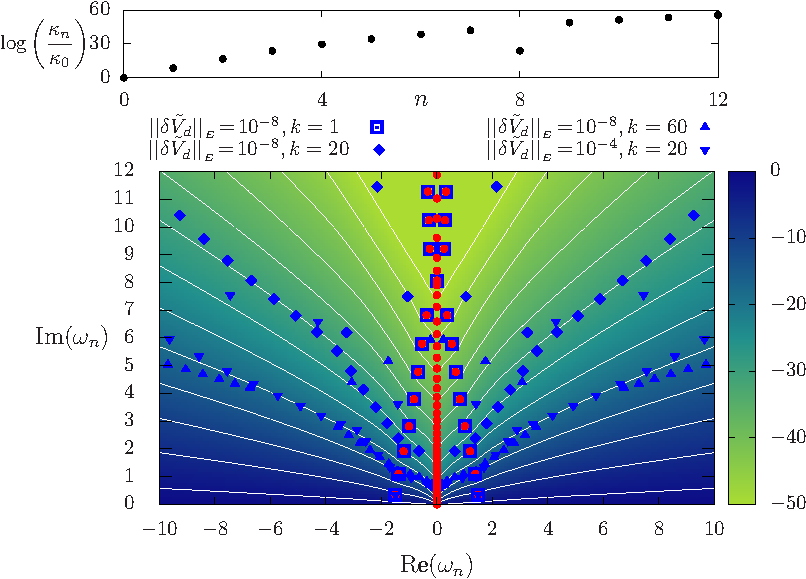
\includegraphics[width={360.00bp},height={252.00bp}]{PseudoSpectra+PertQNM_Schwarzschild}}%
    \gplfronttext
  \end{picture}%
\endgroup

\end{document}
